\documentclass[crop,tikz]{standalone}
\usepackage{tikz}

\makeatletter
\def\namedlabel#1#2{\begingroup
   \def\@currentlabel{#2}%
   \label{#1}\endgroup
}
\makeatother

\newcommand{\ccfNode}[2]{\textbf{#1}:\ #2 \namedlabel{ccf:#1}{Pt. \textbf{#1}}}

\begin{document}
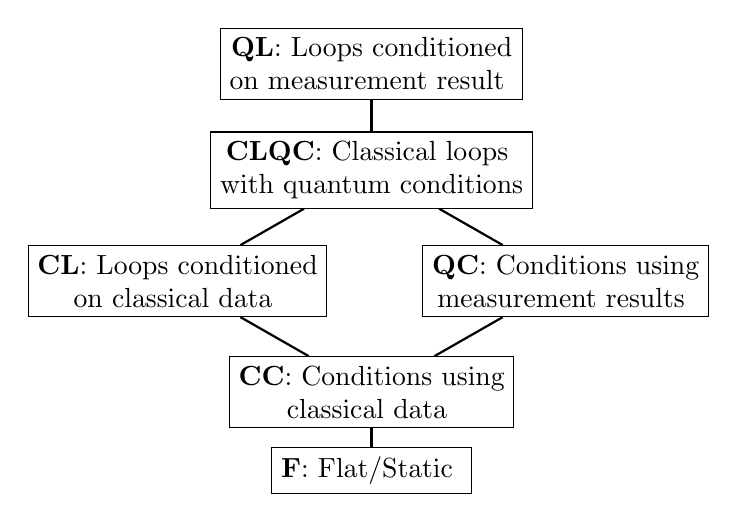
\begin{tikzpicture}
    \node [draw] (ql) at (0,0)                                   [align=center]        {\ccfNode{QL}{Loops conditioned\\ {on measurement result}}};
    \node [draw] [below of=ql]         [yshift=-10]              [align=center] (clqc) {\ccfNode{CLQC}{Classical loops}\\ {with quantum conditions}};
    \node [draw] [below left  of=clqc] [yshift=-20] [xshift=-50] [align=center] (cl)   {\ccfNode{CL}{Loops conditioned\\ {on classical data}}};
    \node [draw] [below right of=clqc] [yshift=-20] [xshift=50]  [align=center] (qc)   {\ccfNode{QC}{Conditions using\\ {measurement results}}};
    \node [draw] [below right of=cl]   [yshift=-20] [xshift=50]  [align=center] (cc)   {\ccfNode{CC}{Conditions using\\ {classical data}}};
    \node [draw] [below of=cc]                                                  (flat) {\ccfNode{F}{Flat/Static}};


    \draw [black, thick] (ql)   -- (clqc);
    \draw [black, thick] (clqc) -- (cl);
    \draw [black, thick] (clqc) -- (qc);
    \draw [black, thick] (cc)   -- (qc);
    \draw [black, thick] (cc)   -- (cl);
    \draw [black, thick] (cc)   -- (flat);
\end{tikzpicture}
\end{document}                 